\section{Mechanism and Ablations}
\label{sec:mechanism}

This section attributes the substrate gain through a per-visit counterfactual, stress-tests the next-region cost against drop-in alternatives, and closes with a methodological note on cross-attention loss-side ablations.

\subsection{Per-visit context counterfactual (five states)}
\label{subsec:mechanism-pervisit}

To isolate per-visit context, we compare canonical Check2HGI against POI-pooled Check2HGI (canonical vectors mean-pooled per POI and applied uniformly to every visit, killing per-visit variation while preserving the training signal). Canonical vs.\ pooled isolates per-visit context; pooled vs.\ HGI isolates the contrastive training signal.

Under the matched-head GRU single-task ceiling, the substrate gap (canonical $-$ HGI) splits consistently at all five states (Figure~\ref{fig:per-visit}): per-visit context dominates at every state, with both components positive. Paired Wilcoxon signed-rank tests reach the $n=5$ ceiling at AL and AZ ($p=0.0312$, $5/5$ folds positive); FL/CA/TX show the same monotone ordering at all five per-fold pairs. A two-band pattern emerges across state scale: at small states (AL ${\sim}72\,\%$, AZ ${\sim}64\,\%$) the training-signal residual is 28--36\,\%; at large states (FL/CA/TX, ${\sim}89$--$90\,\%$) the pooled embeddings collapse almost entirely to the HGI level, leaving ${\sim}10\,\%$ to the training signal. This is consistent with large transition graphs (4.7k--8.5k regions) providing weaker per-POI contrastive signal, so Check2HGI's advantage at large states is almost entirely in the per-visit contextual variation it introduces.

\begin{figure}[t]
\centering
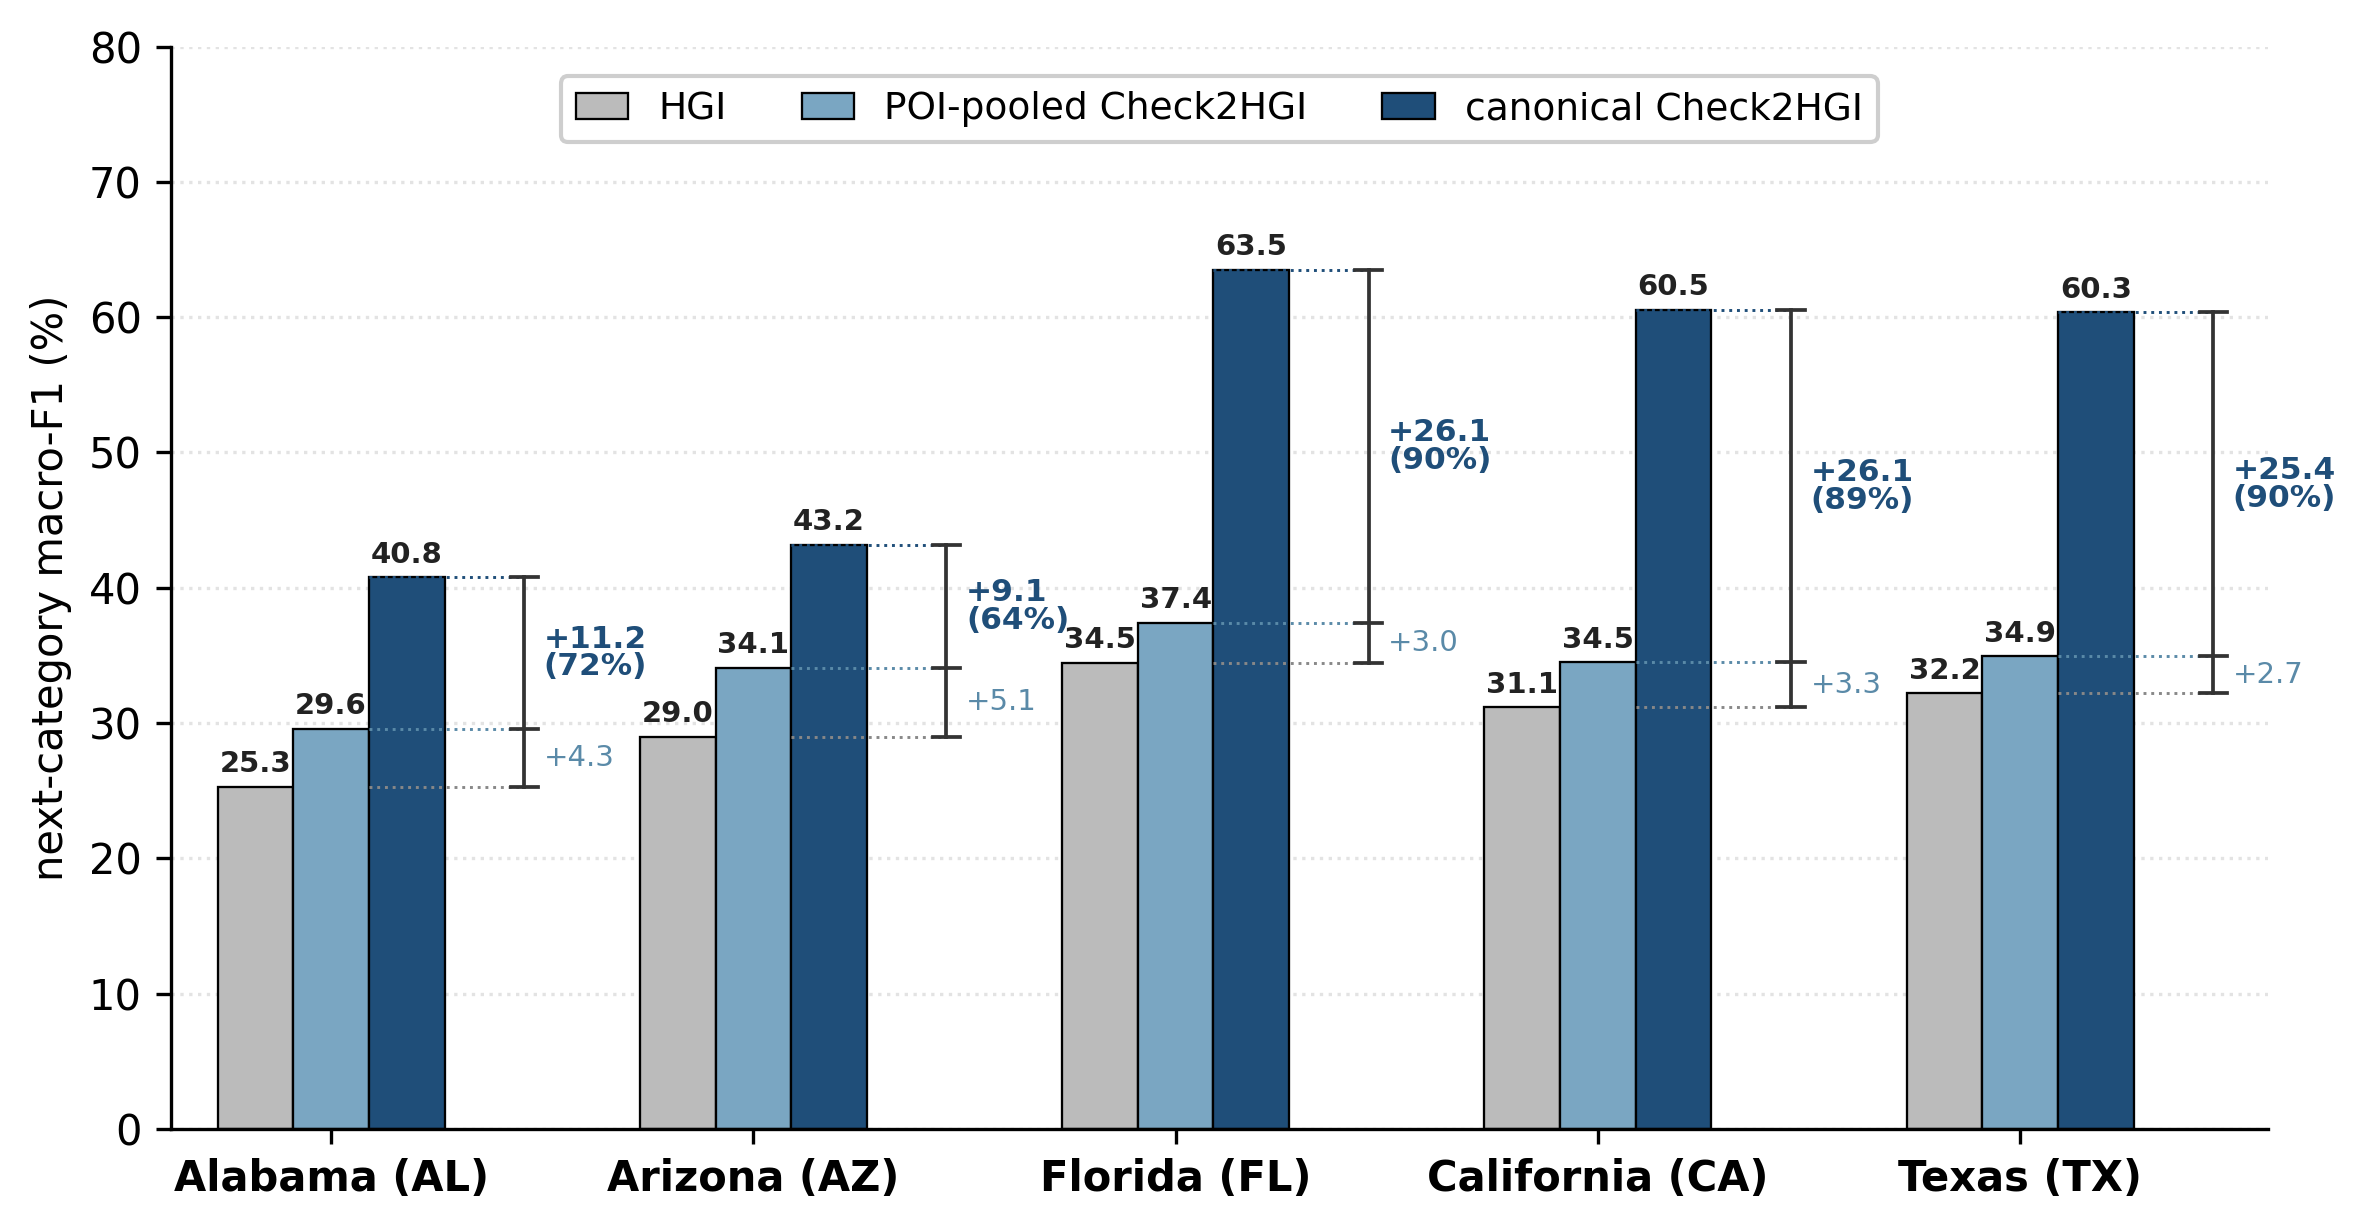
\includegraphics[width=\linewidth]{figs/per-visit.png}
\caption{Per-visit context decomposition at five states under the matched-head GRU STL ceiling. The substrate gap (canonical Check2HGI $-$ HGI) splits into a per-visit component (canonical $-$ POI-pooled) and a training-signal component (POI-pooled $-$ HGI). Per-state shares are reported in \S\ref{subsec:mechanism-pervisit}.}
\label{fig:per-visit}
\end{figure}


\subsection{Drop-in MTL ablations do not recover the next-region cost}
\label{subsec:mechanism-ablations}

The next-region cost is sign-consistent across all five states ($7$ to $17$ pp on Acc@10). At FL we tried three drop-in replacements (FAMO~\cite{liu2023famo}, a magnitude balancer; Aligned-MTL~\cite{senushkin2023aligned}, a direction-aligning balancer; and a hierarchical-additive-softmax region head) with substrate, backbone, optimiser and schedule fixed at \S\ref{sec:method}. None reached the $+3$ pp Acc@10 recovery target or paired-Wilcoxon $p_{\text{greater}}<0.10$; the strongest, the hierarchical head, reaches only ${\approx}+1.7$ pp. The cost stays intact, suggesting a structural cost of the cross-attention interaction with the region head rather than a loss-recipe artefact.

\subsection{Cross-attention $\lambda = 0$ is not encoder isolation}
\label{subsec:mechanism-isolation}

A natural ablation zeros one task's weight in Eq.~\eqref{eq:loss}, on the assumption that $\lambda_{\text{cat}}=0$ or $\lambda_{\text{reg}}=0$ ablates the corresponding encoder. Under cross-attention this is unsound: the targeted encoder still updates through the key/value projections of the surviving stream, so its parameters co-adapt to the surviving task. A targeted probe at AZ quantifies the gap: encoder-frozen isolation reaches region Acc@10 $60.72$, while loss-side $\lambda_{\text{cat}}=0$ reaches $62.70$ on the same folds, a $+1.98$ pp lift driven through the K/V projections. We therefore use \textbf{encoder-frozen isolation} (targeted encoder random-init, frozen) throughout; the caution generalises to any cross-task attention multi-task model.
